\chapter{Hamiltonian Path/Cycle}
Ajur was walking with Jura thinking how a walk could be named after him. Rishnak found Ajur to be an interesting person to discuss puzzles related to Graph Theory. After the Eulerian Walk, Rishnak thought of another closely related walk- namely Hamiltonian Path and Hamiltonian Cycle. A Hamiltonian Path is a path in which all the vertices are visited exactly once. The length of a path is the number of edges in that path. A Hamiltonian path in a graph with $n$ vertices will have a path length of $n-1$, A Hamiltonian cycle is a cycle that visits each vertex once and only once. The length of Hamiltonian Cycle in a graph with $n$ vertices will have a length of $n$. Rishnak asked Ajur whether there is a Hamiltonian Cycle in the following graph Figure \ref{5g1},
\begin{figure}
\begin{center}
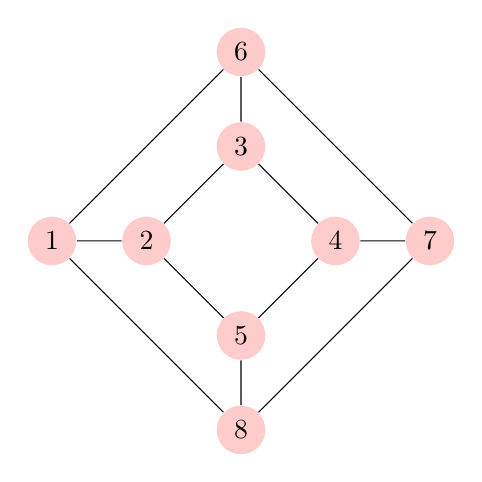
\begin{tikzpicture}
  [scale=.6,auto=left,every node/.style={circle,fill=red!20}]
  \node (n1) at (1,7) {1};
  \node (n2) at (3,7)  {2};
  \node (n4) at (7,7) {4};
  \node (n7) at (9,7)  {7};
  \node (n6) at (5,11)  {6};
   \node (n3) at (5,9) {3};
   \node (n5) at (5,5) {5};
   \node (n8)  at (5,3) {8};
  \foreach \from/\to in {n1/n2,n2/n3,n3/n4,n4/n5,n5/n2,n1/n6,
  n6/n7, n7/n8, n8/n1, n3/n6, n4/n7, n5/n8}
    \draw (\from) -- (\to);

\end{tikzpicture}
\caption{ Cube Graph }\label{5g1}
\end{center}
\end{figure}

Ajur thought about for a few seconds and he drew the Hamiltonian cycle of Figure \ref{5g1} in Figure \ref {5g2}

\begin{figure}
\begin{center}
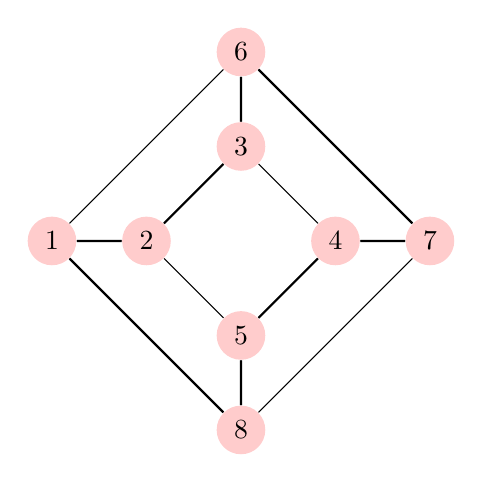
\begin{tikzpicture}
  [scale=.6,auto=left,every node/.style={circle,fill=red!20}]
  \node (n1) at (1,7) {1};
  \node (n2) at (3,7)  {2};
  \node (n4) at (7,7) {4};
  \node (n7) at (9,7)  {7};
  \node (n6) at (5,11)  {6};
   \node (n3) at (5,9) {3};
   \node (n5) at (5,5) {5};
   \node (n8)  at (5,3) {8};
  \foreach \from/\to in {n1/n2,n2/n3,n3/n4,n4/n5,n5/n2,n1/n6,
  n6/n7, n7/n8, n8/n1, n3/n6, n4/n7, n5/n8}
    \draw (\from) -- (\to);
\path[thick] (n1) edge (n2)
(n2) edge (n3)
(n3) edge (n6)
(n6) edge (n7)
(n7) edge (n4)
(n4) edge (n5)
(n5) edge (n8)
(n8) edge (n1);
\end{tikzpicture}
\caption{ Cube Graph with Hamiltonian  Cycle marked in thick edges}\label{5g2}
\end{center}
\end{figure}

Rishnak mentioned that the problem started when mathematician Hamilton wanted a cycle to visit all the vertices of a Dodecahedron (another platonic solid, like cube) which has 20 vertices and 30 edges. 
